% -*- TeX -*-
\documentclass[aspectratio=169]{beamer}

\usepackage{listings}
\usepackage{amsmath}
\usepackage{array}
\usepackage{tikz}

\usetikzlibrary{decorations.pathreplacing}
\usetikzlibrary{fit,matrix}
\usetikzlibrary{shapes,calc}

\title{Crustal Deformation Modeling Tutorial}
\subtitle{Using Gravity and Initial Stresses}
\author{Charles Williams \\
  Brad Aagaard \\
  Matthew Knepley}
\institute{
\includegraphics[scale=0.4]{../../logos/cig_blackfg}}
\date{June 11, 2019}


% ---------------------------------------------------- CUSTOMIZATION
\renewcommand{\thispdfpagelabel}[1]{}
\newcommand{\pylith}[1]{{\color{green}#1}}
\newcommand{\python}[1]{{\color{red}#1}}
\usetheme{CIG}
% Style information for PyLith presentations.

% Colors
\definecolor{ltorange}{rgb}{1.0, 0.74, 0.41} % 255/188/105
\definecolor{orange}{rgb}{0.96, 0.50, 0.0} % 246/127/0

\definecolor{ltred}{rgb}{1.0, 0.25, 0.25} % 255/64/64
\definecolor{red}{rgb}{0.79, 0.00, 0.01} % 201/0/3

\definecolor{ltpurple}{rgb}{0.81, 0.57, 1.00} % 206/145/255
\definecolor{purple}{rgb}{0.38, 0.00, 0.68} % 97/1/175

\definecolor{ltblue}{rgb}{0.2, 0.73, 1.0} % 51/187/255
\definecolor{mdblue}{rgb}{0.28, 0.50, 0.80} % 72/128/205
\definecolor{blue}{rgb}{0.12, 0.43, 0.59} % 30/110/150

\definecolor{ltltgreen}{rgb}{0.7, 1.00, 0.7} % 96/204/14
\definecolor{ltgreen}{rgb}{0.37, 0.80, 0.05} % 96/204/14
\definecolor{green}{rgb}{0.23, 0.49, 0.03} % 59/125/8
  
\definecolor{dkslate}{rgb}{0.18, 0.21, 0.28} % 47/53/72
\definecolor{mdslate}{rgb}{0.45, 0.50, 0.68} % 114/127/173
\definecolor{ltslate}{rgb}{0.85, 0.88, 0.95} % 216/225/229


\newcommand{\includefigure}[2][]{{\centering\includegraphics[#1]{#2}\par}}
\newcommand{\highlight}[1]{{\bf\usebeamercolor[fg]{structure}#1}}
\newcommand{\important}[1]{{\color{red}#1}}
\newcommand{\issue}[2]{\item[Issue:] {\color{red}#1}\\{\item[Soln:] \color{blue}#2}\\[4pt]}

\setbeamercolor{alerted text}{fg=ltgreen}
\setbeamertemplate{description item}[align left]


\newcommand{\lhs}[1]{{\color{blue}#1}}
\newcommand{\rhs}[1]{{\color{red}#1}}
\newcommand{\annotateL}[2]{%
  {\color{blue}\underbrace{\color{blue}#1}_{\color{blue}\mathclap{#2}}}}
\newcommand{\annotateR}[2]{%
  {\color{red}\underbrace{\color{red}#1}_{\color{red}\mathclap{#2}}}}
\newcommand{\eqnannotate}[2]{%
  {\color{blue}%
  \underbrace{\color{black}#1}_{\color{blue}\mathclap{#2}}}}

\newcommand{\trialvec}[1][]{{\vec{\psi}_\mathit{trial}^{#1}}}
\newcommand{\trialscalar}[1][]{{\psi_\mathit{trial}^{#1}}}
\newcommand{\basisvec}[1][]{{\vec{\psi}_\mathit{basis}^{#1}}}
\newcommand{\basisscalar}[1][]{{\psi_\mathit{basis}^{#1}}}

\newcommand{\tensor}[1]{\bm{#1}}
\DeclareMathOperator{\Tr}{Tr}

\usefonttheme[onlymath]{serif}

% minted shortcuts
\newminted{cfg}{bgcolor=ltslate,autogobble,fontsize=\tiny}
\newminted{bash}{bgcolor=ltltgreen,autogobble,fontsize=\tiny}

% PyLith components
\newcommand{\pylith}[1]{{\ttfamily\color{magenta}#1}}



% ========================================================= DOCUMENT
\begin{document}

% ------------------------------------------------------------ SLIDE
\maketitle

% ------------------------------------------------------------ SLIDE
\logo{
\includegraphics[height=4.5ex]{../../logos/cig_blackfg}}

% ========================================================== SECTION
\section{Gravitational body forces}

% ========================================================== SUBSECTION
\subsection{Concepts covered}
% ------------------------------------------------------------ SLIDE
\begin{frame}
  \frametitle{Concepts Covered in this Session}
  \summary{}

  \begin{itemize}
  \item When are gravitational stresses necessary?
  \item Usage of gravitational body forces in 2D
  \item Usage of reference stresses to balance body forces
  \item Usage of incompressible elasticity to achieve a reference
    state
  \item Usage of traction boundary conditions to represent a surface
    load
  \end{itemize}

  
\end{frame}


% ========================================================== SUBSECTION
\subsection{When is gravity needed?}

% ------------------------------------------------------------ SLIDE
\begin{frame}
  \frametitle{When Do We Need to Use Gravitational Stresses?}
  \summary{}

  \begin{itemize}
  \item Pressure/stress-dependent rheology
    \begin{itemize}
    \item Pressure-dependent bulk rheology (e.g., plasticity)
    \item Stress-dependent fault rheology (e.g., friction)
    \end{itemize}
  \item Viscoelastic simulations where we care about vertical
    deformation
  \item Other simulations where we care about the absolute stress
    state
  \end{itemize}
  
\end{frame}

% ========================================================== SECTION
\subsection{2-D gravity examples}

% ------------------------------------------------------------ SLIDE
\begin{frame}
  \frametitle{Two-dimensional Gravity Simulations}
  \summary{}

  \vfill
  Files are in {\tt\color{red} examples/2d/reverse}.
  None of these problems involve faulting.
  \vfill

\begin{enumerate}
\item {\tt\color{red} step01} Use gravitational body forces with no
  reference stresses.
  \begin{itemize}
  \item Entire domain deforms vertically since material is
    compressible.
  \end{itemize}
\item {\tt\color{red} step02} Use gravitational body forces
  and balance them with analytically-determined reference stresses.
  \begin{itemize}
  \item Stresses are reasonably-well balanced and there is much less
    deformation.
  \end{itemize}
\item {\tt\color{red} step03} Use gravitational body forces for an
  incompressible elastic material.
  \begin{itemize}
  \item Stresses are nearly isotropic and there is virtually no
    deformation.
  \end{itemize}
\item {\tt\color{red} step04} Use traction boundary conditions
  to represent a surface load.
  \begin{itemize}
  \item Primarily vertical deformation centered beneath the applied
    load.
  \end{itemize}
\end{enumerate}

\end{frame}


% ========================================================== SECTION
\subsection{Step 1}

% ------------------------------------------------------------ SLIDE
\begin{frame}
  \frametitle{Step 1}
  \summary{Gravitational body forces applied to elastic material}

  \vfill
  \begin{center}
      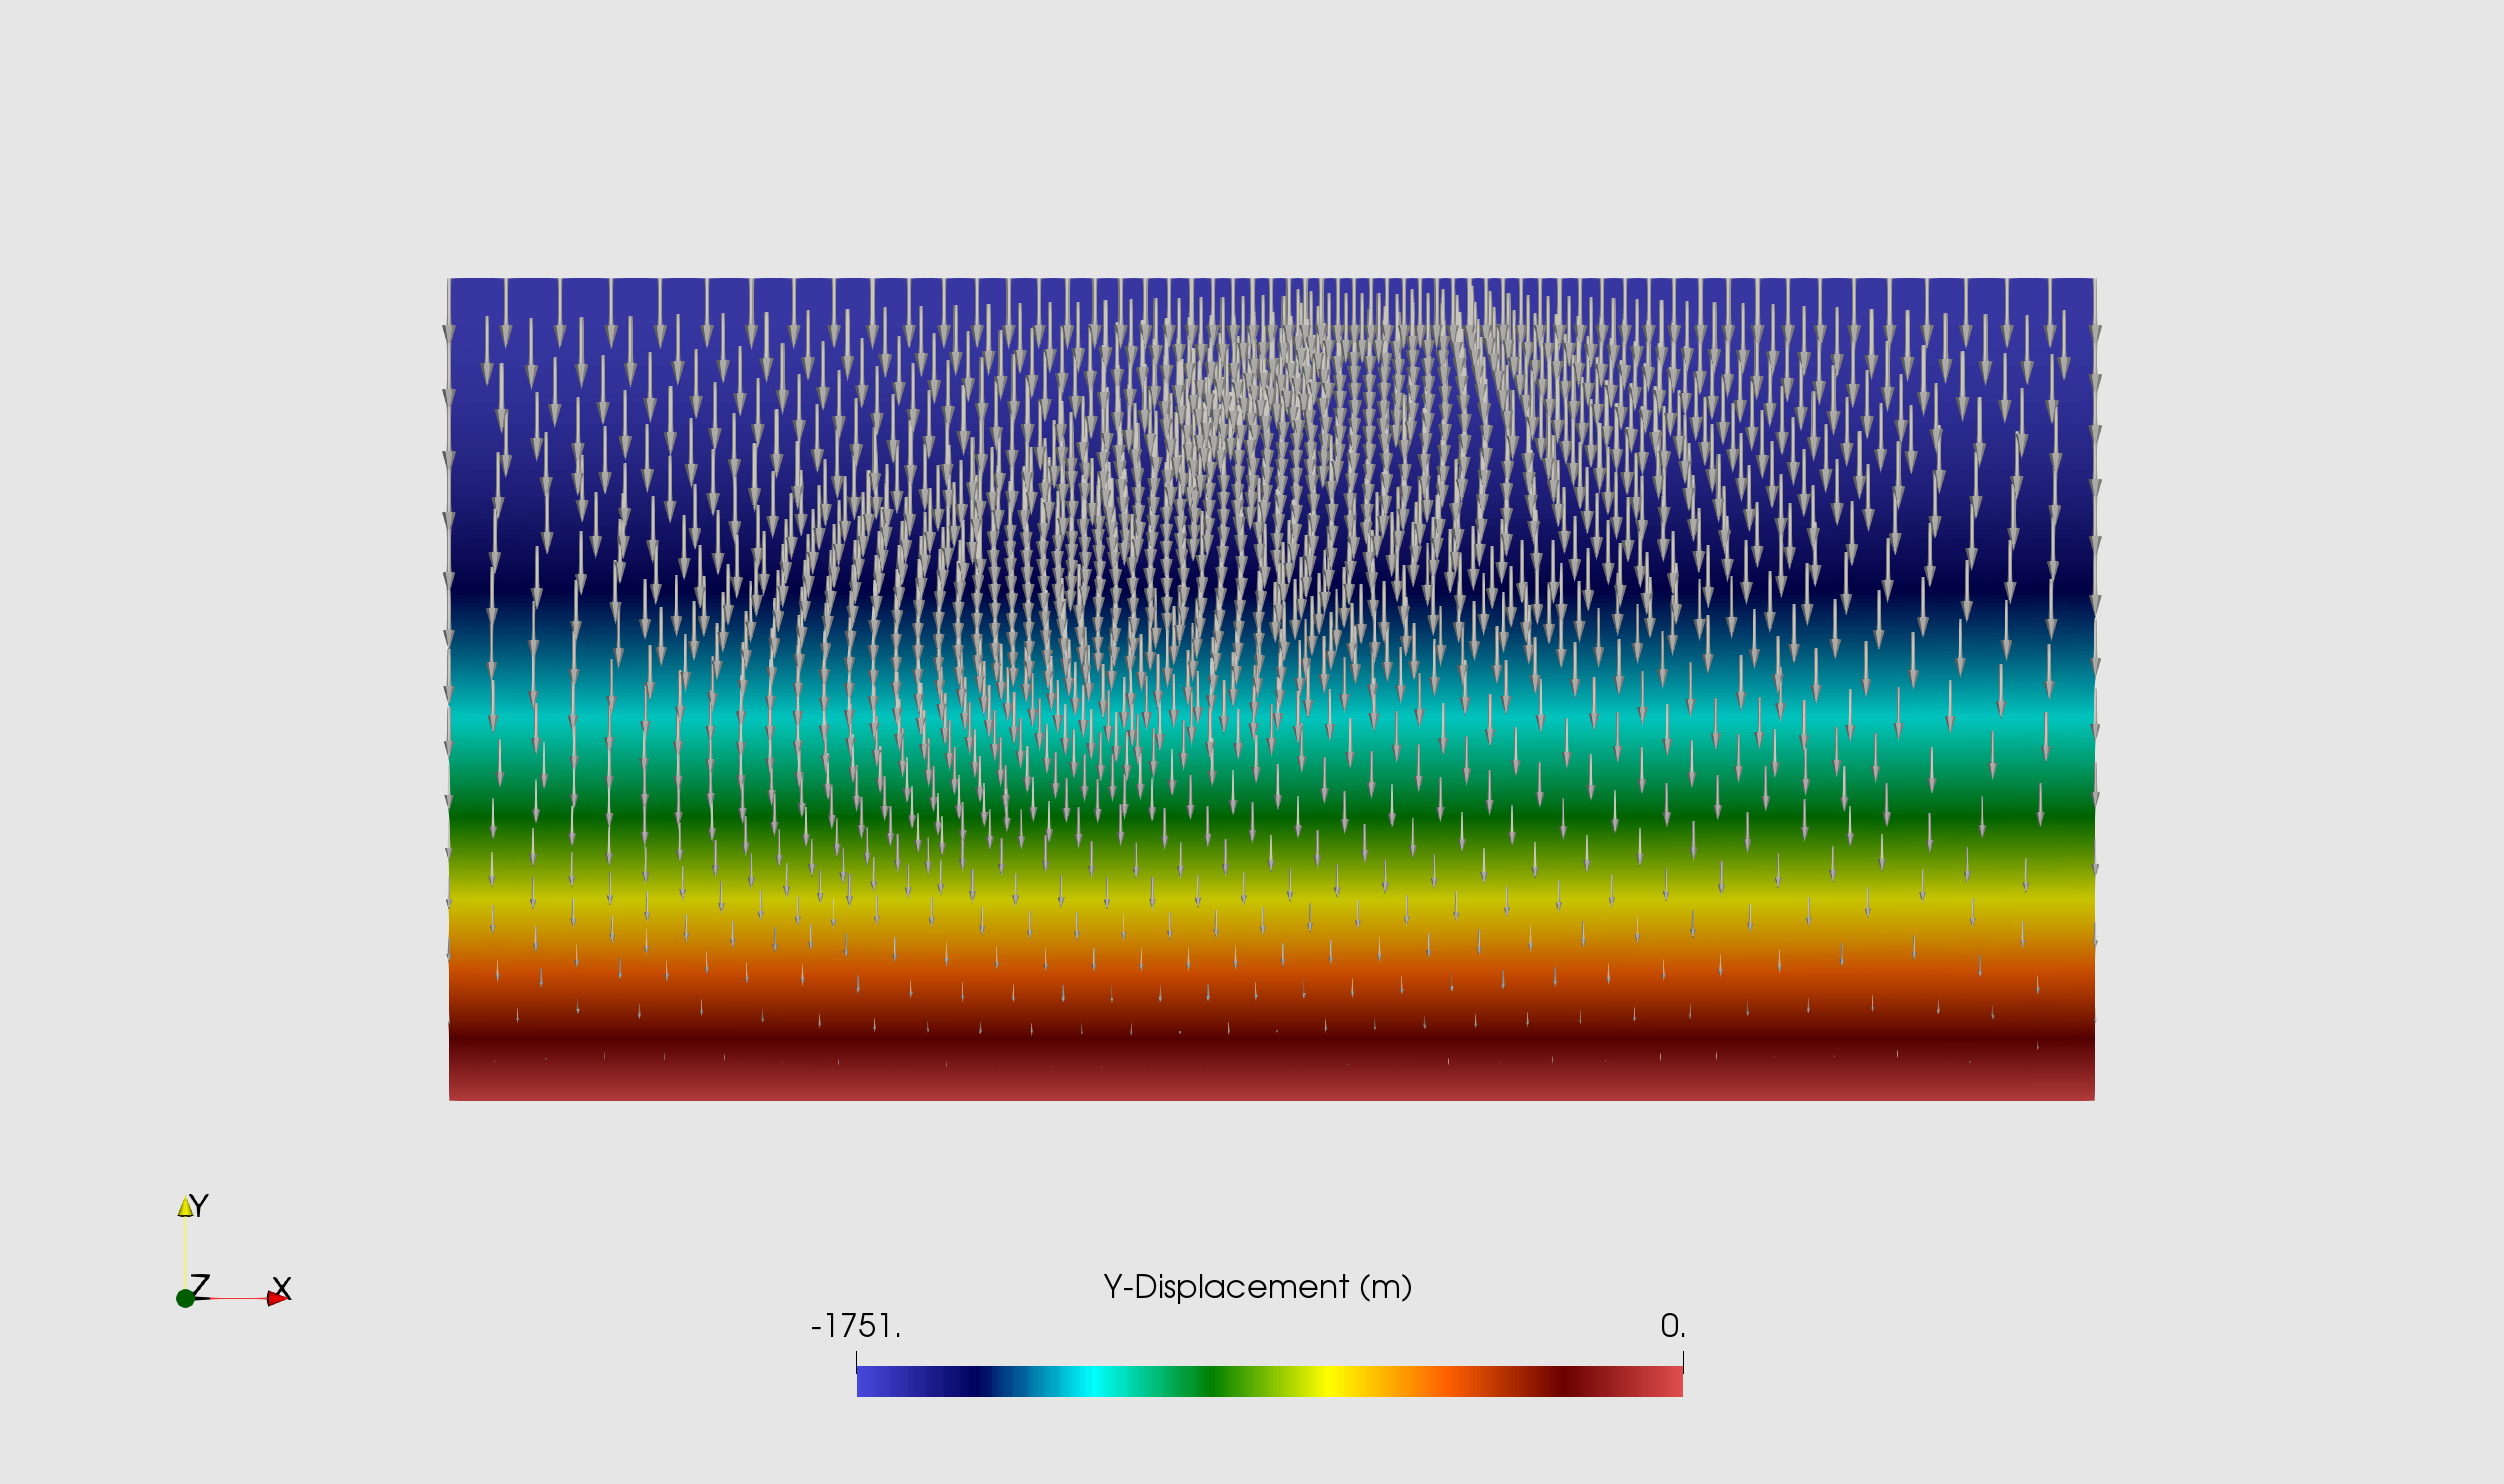
\includegraphics[height=6.1cm]{figs/reverse_step01_displ}
  \end{center}
\vfill
      
\end{frame}


% ========================================================== SECTION
\subsection{Step 2}

% ------------------------------------------------------------ SLIDE
\begin{frame}
  \frametitle{Step 2}
  \summary{Gravitational body forces with reference stress}

  \vfill
  \begin{center}
      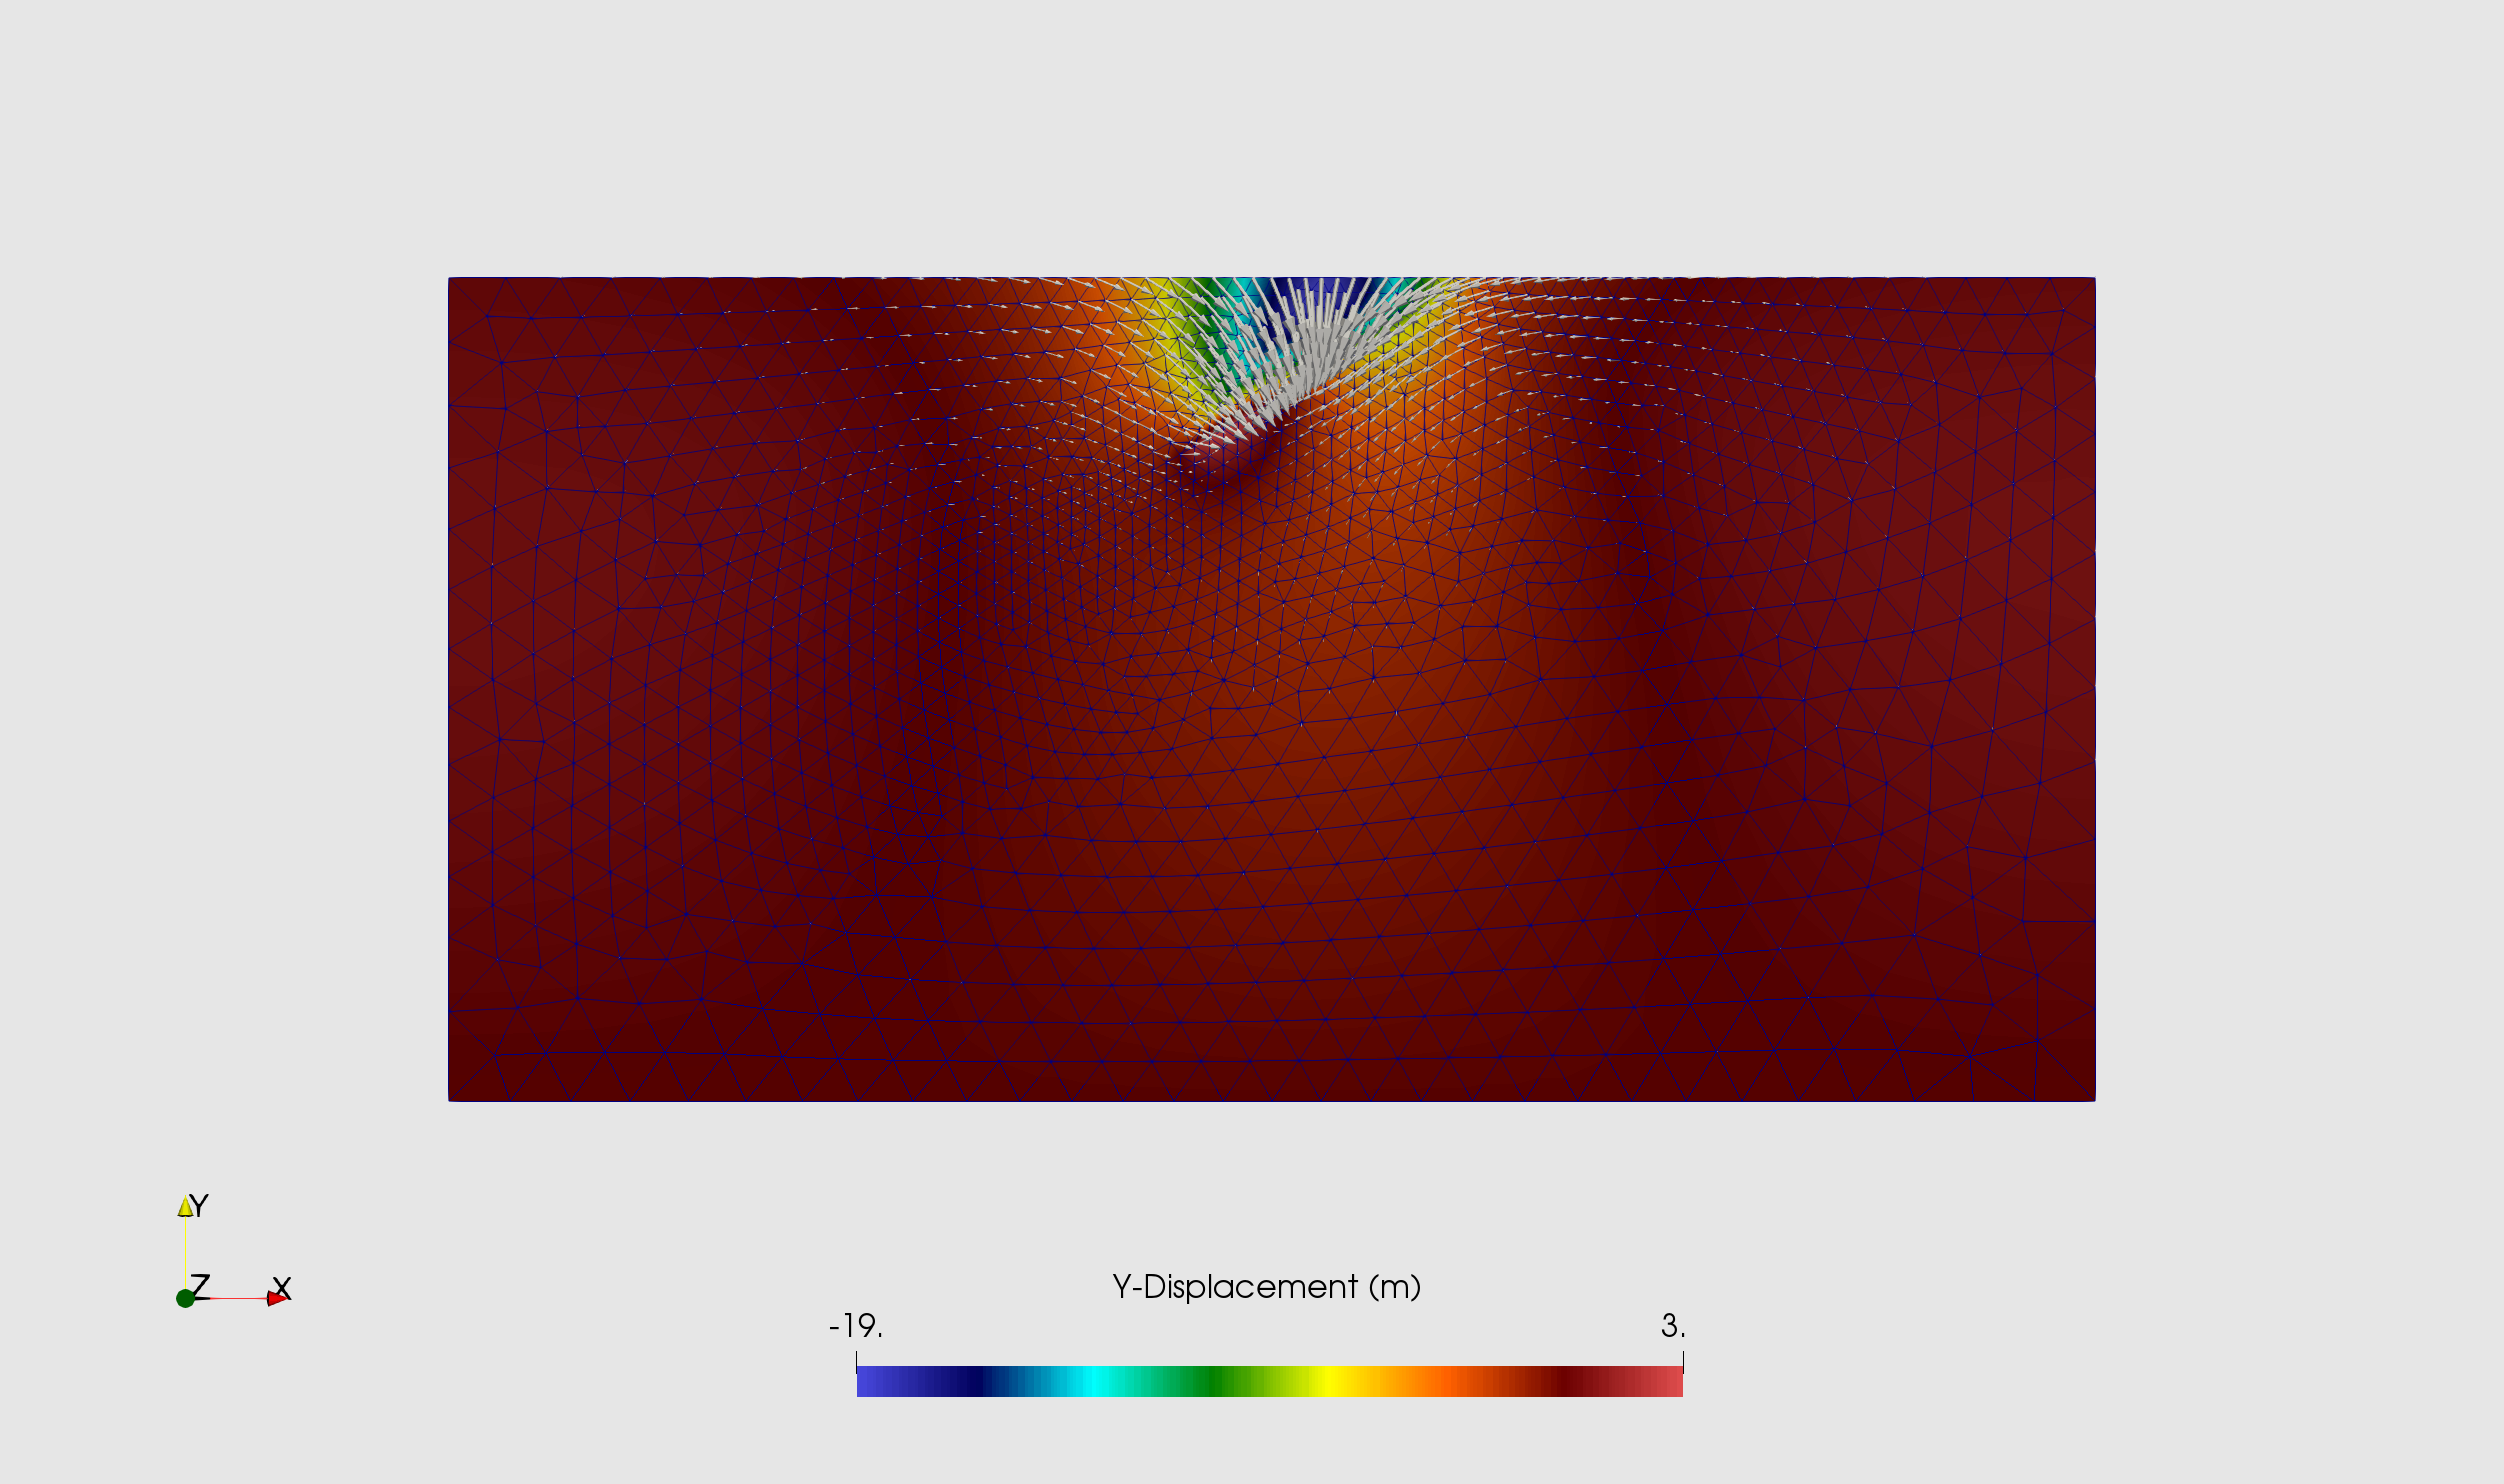
\includegraphics[height=6.1cm]{figs/reverse_step02_displ}
  \end{center}
\vfill
      
\end{frame}


% ========================================================== SECTION
\subsection{Step 3}

% ------------------------------------------------------------ SLIDE
\begin{frame}
  \frametitle{Step 3}
  \summary{Gravitational body forces applied to incompressible elastic
    material}

  \vfill
  \begin{center}
      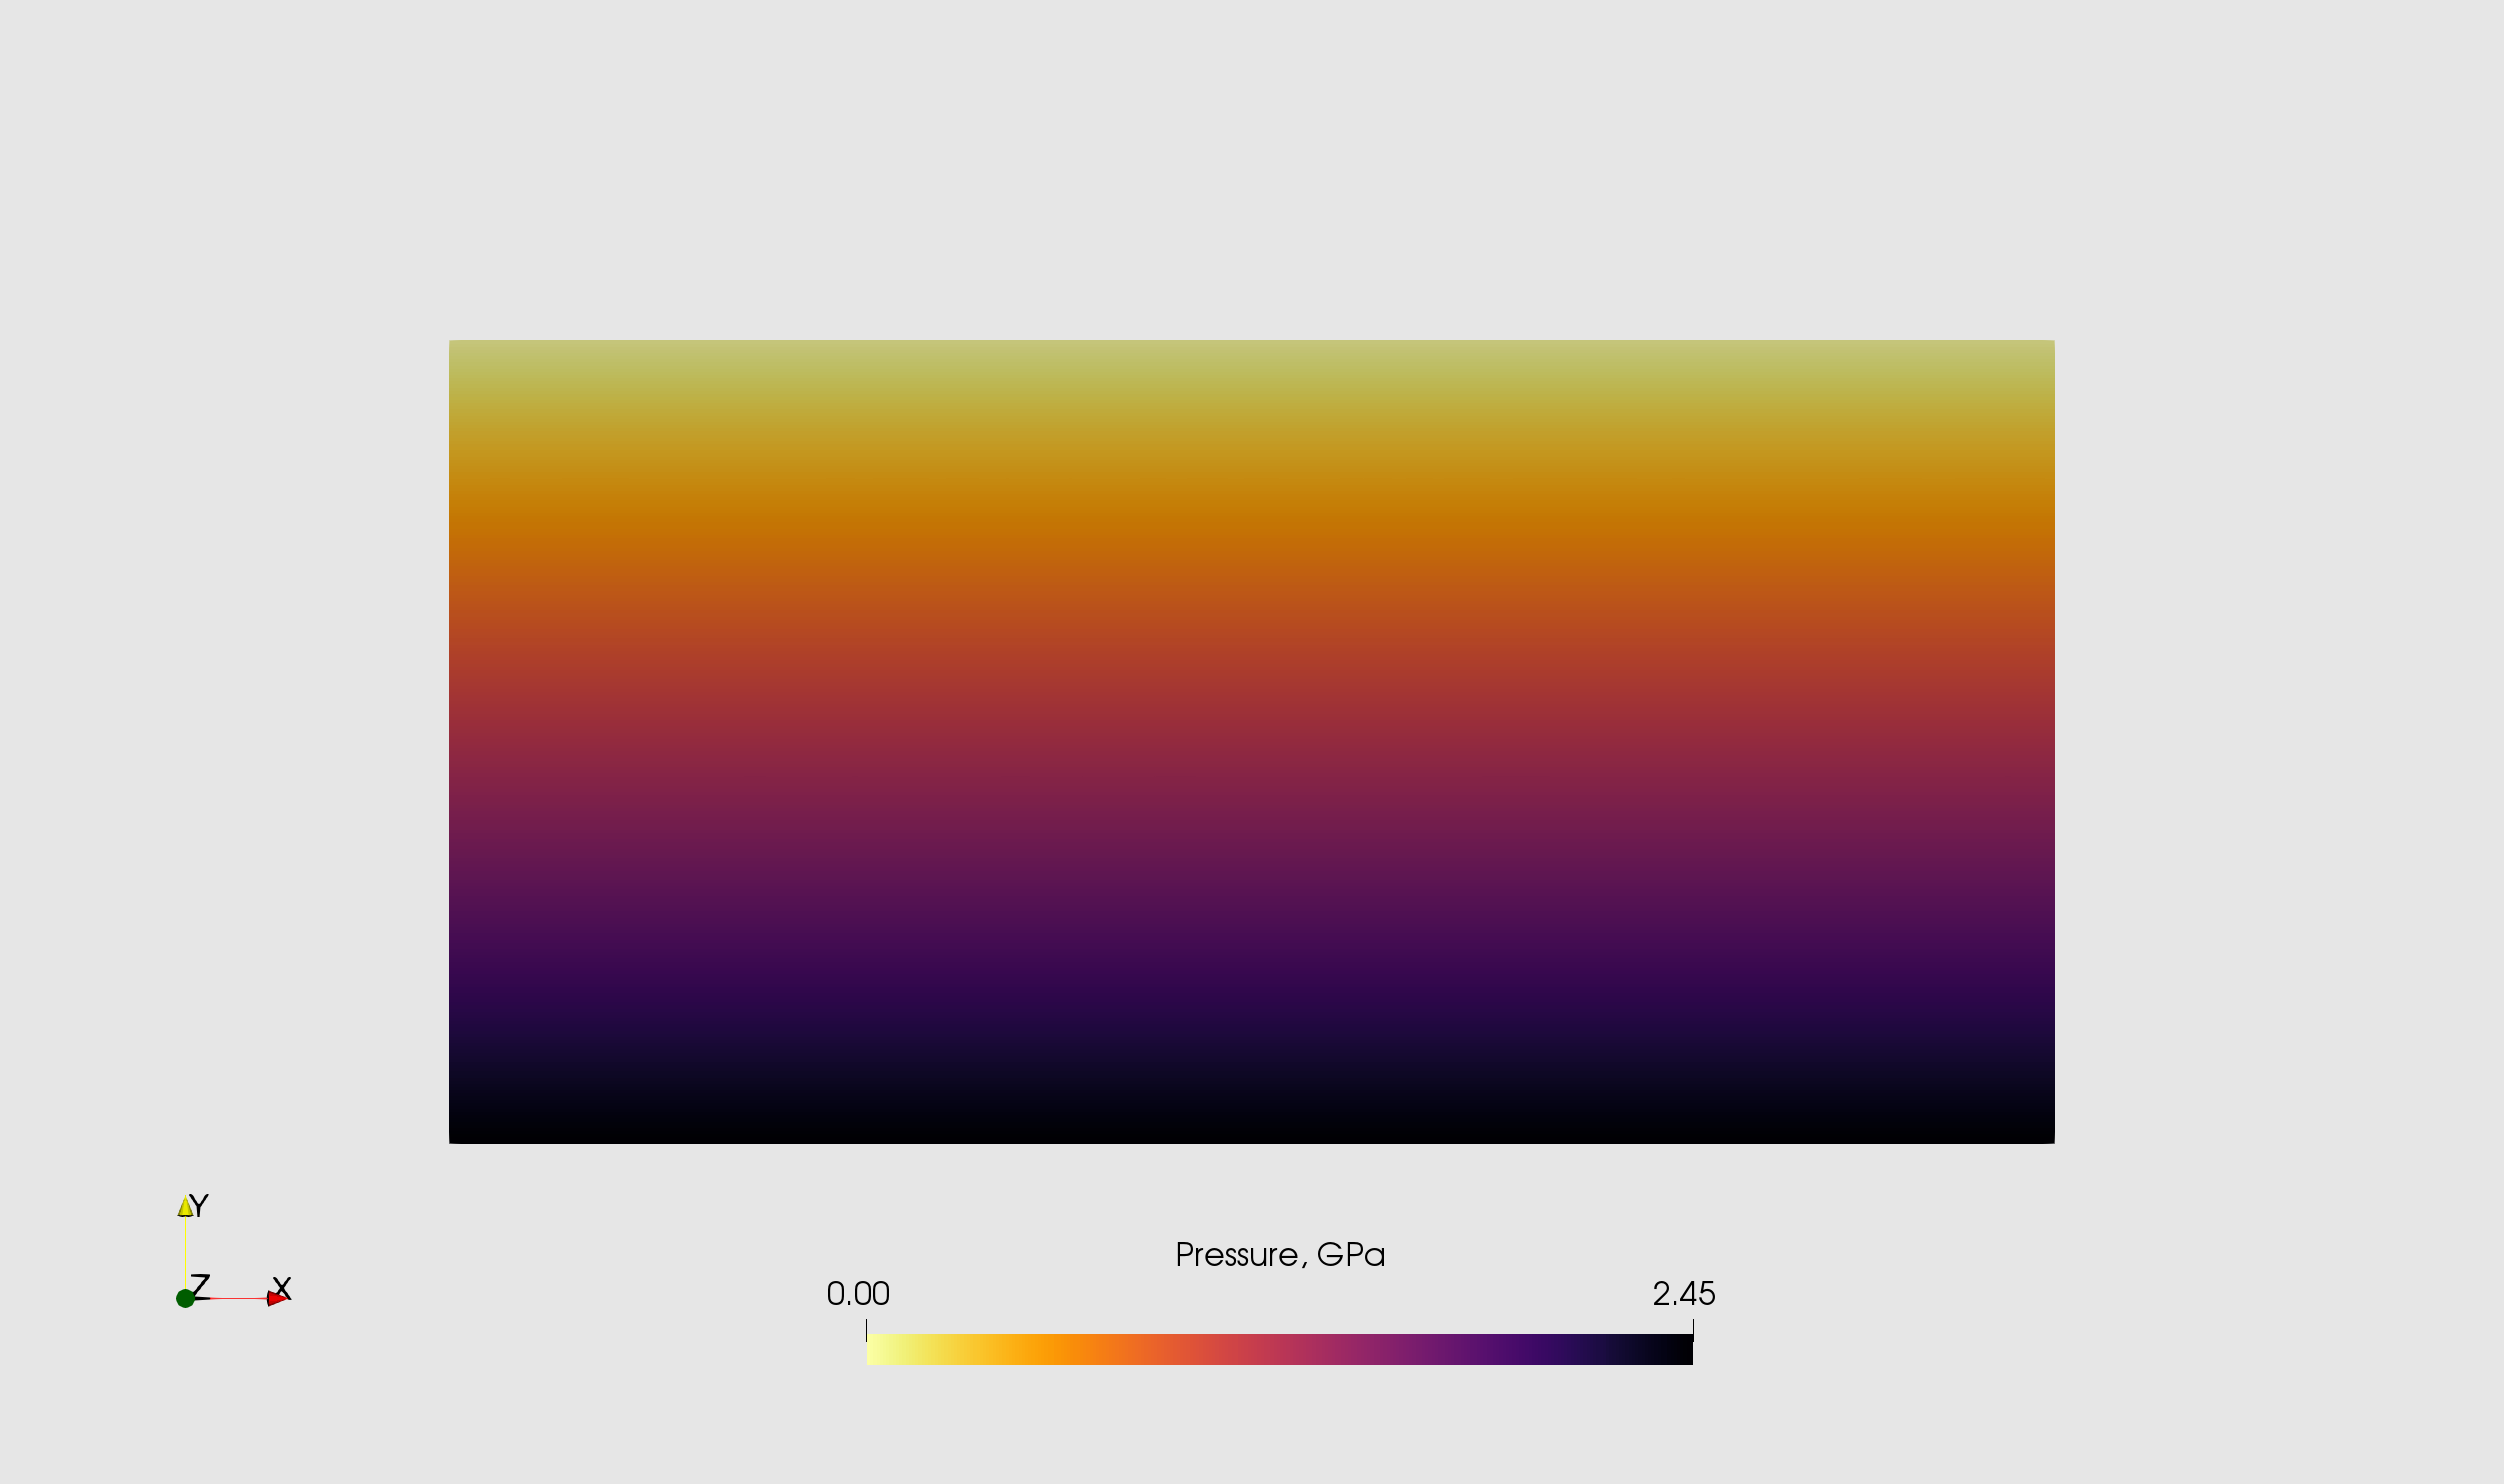
\includegraphics[height=6.1cm]{figs/reverse_step03_pres}
  \end{center}
\vfill
      
\end{frame}


% ========================================================== SECTION
\subsection{Step 4}

% ------------------------------------------------------------ SLIDE
\begin{frame}
  \frametitle{Step 4}
  \summary{Normal tractions applied to simulate a surface load}

  \vfill
  \begin{center}
      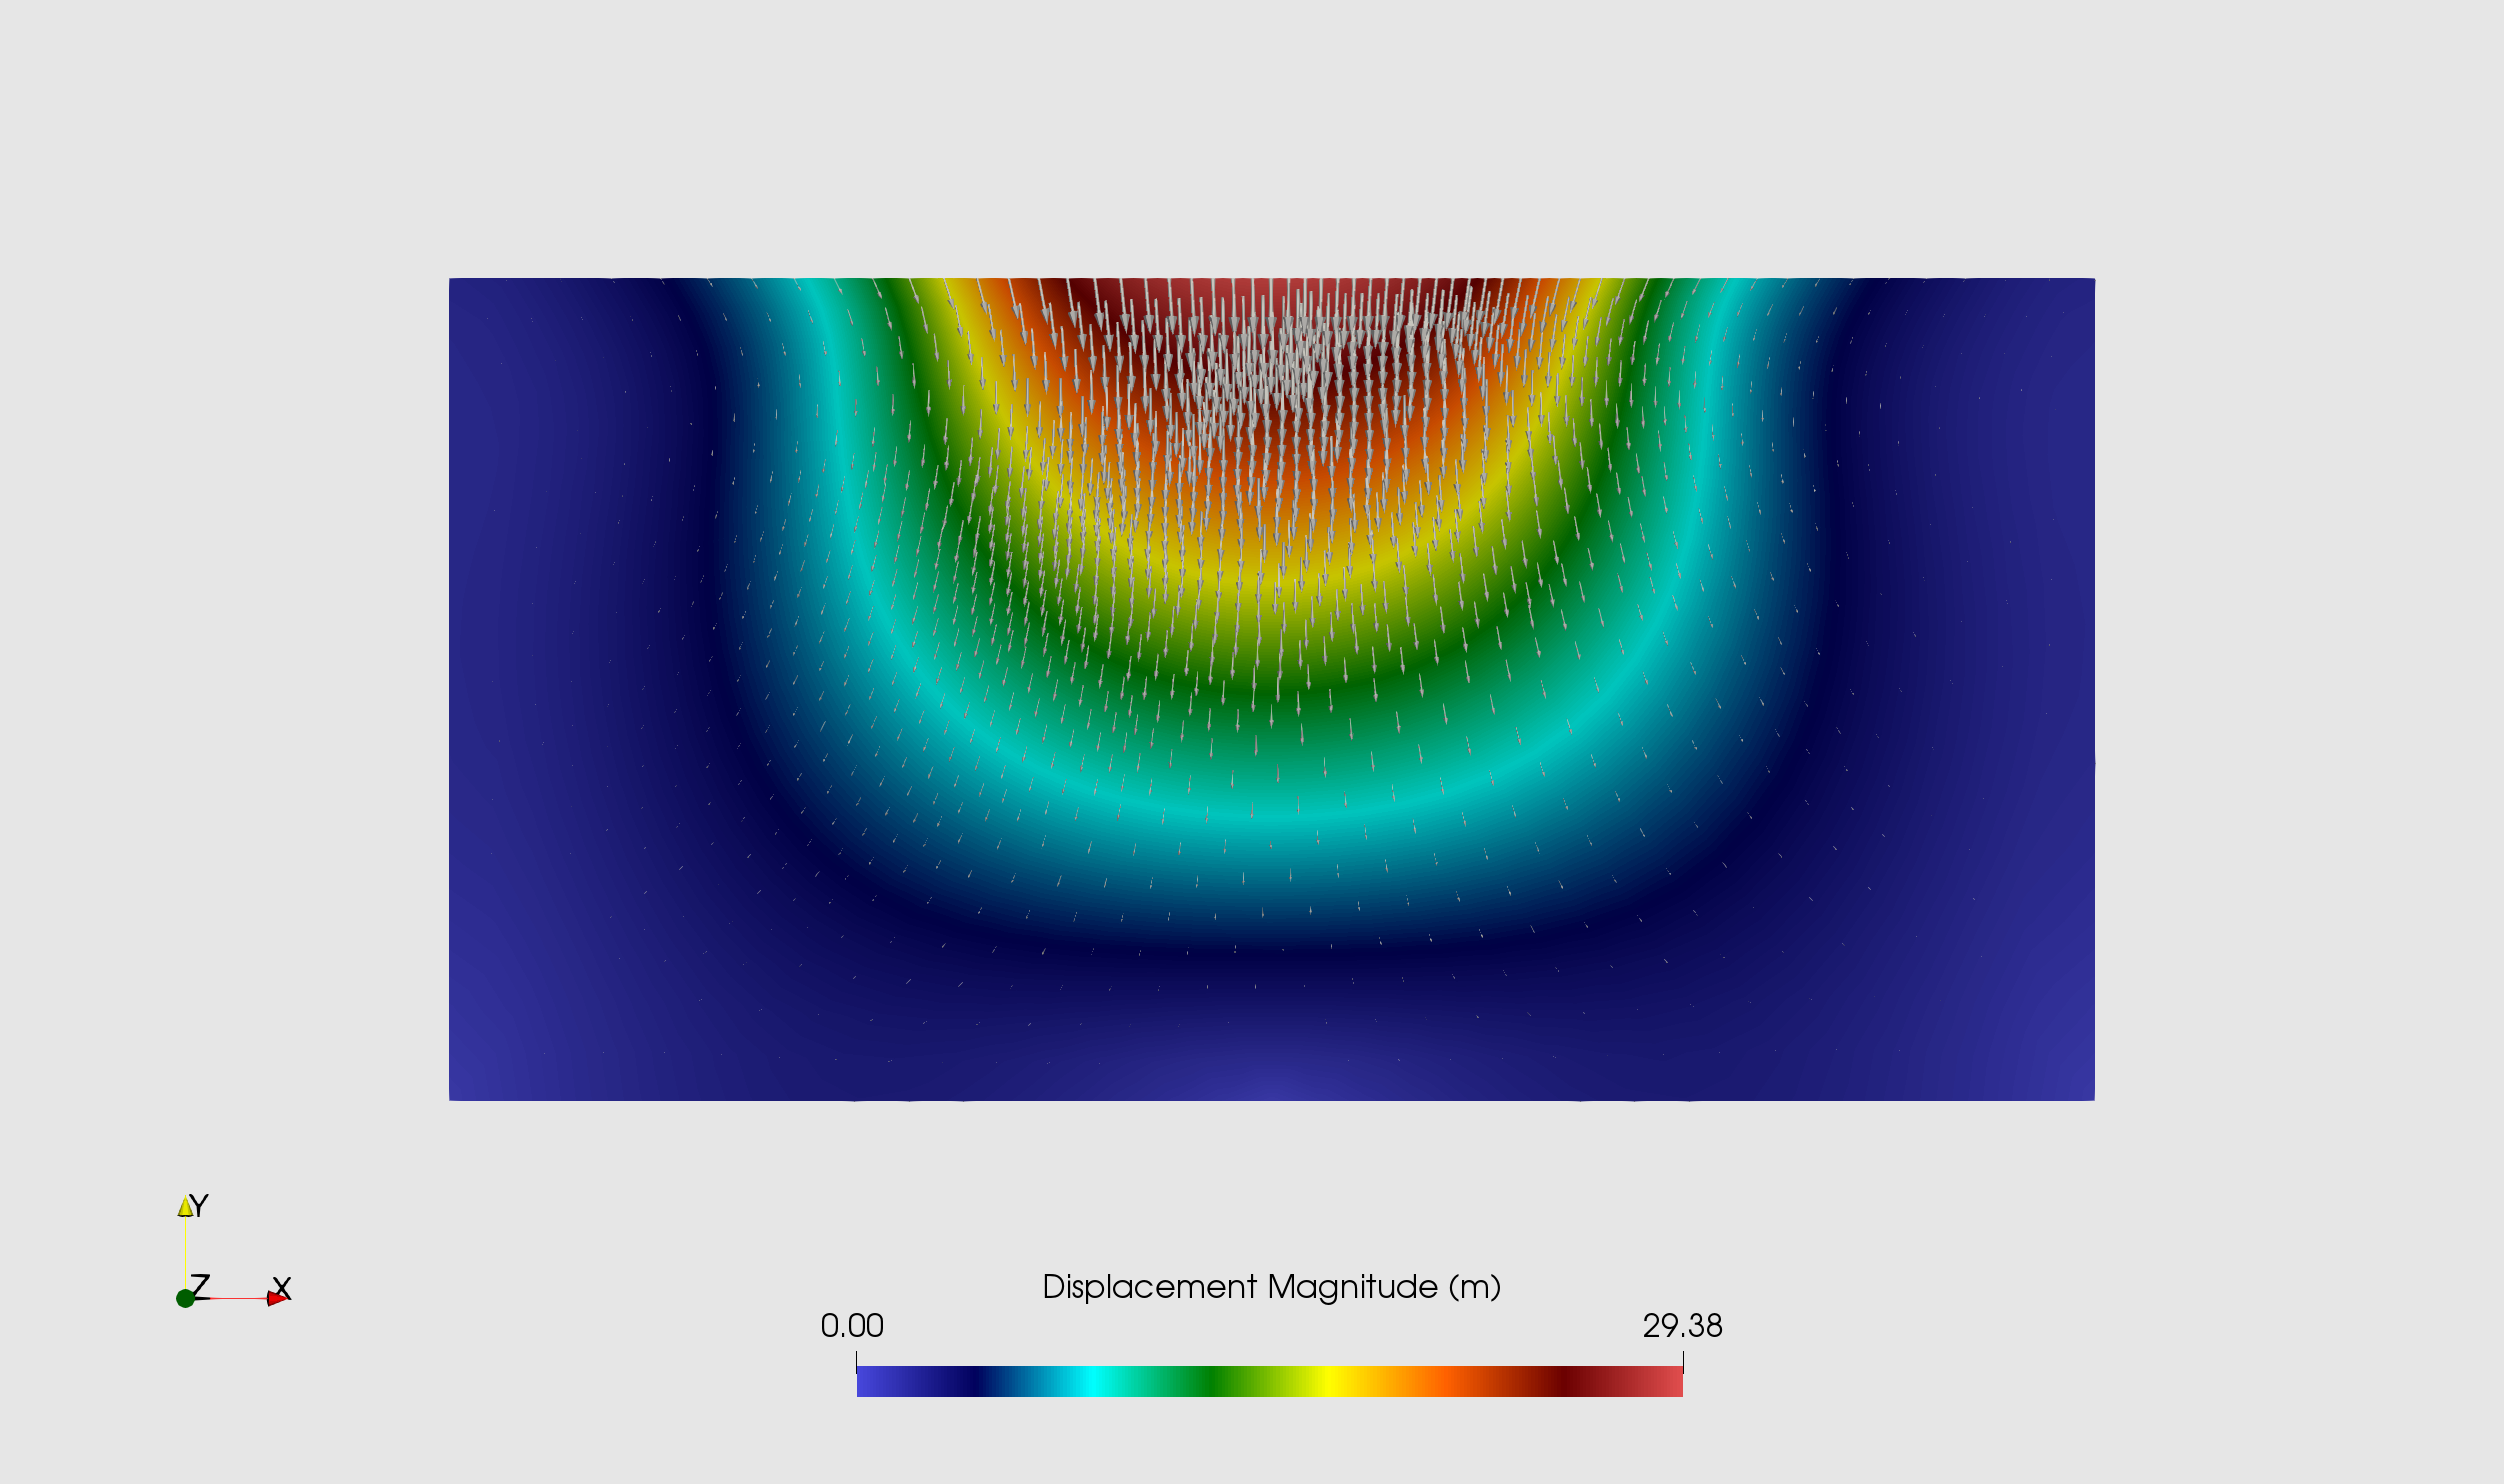
\includegraphics[height=6.1cm]{figs/reverse_step04_displ}
  \end{center}
\vfill
      
\end{frame}


% ======================================================================
\end{document}


% End of file
